%\PassOptionsToPackage{demo}{graphicx}
\PassOptionsToPackage{table}{xcolor}
\documentclass[portrait,final,a0paper,fontscale=0.310]{baposter}
\usepackage[utf8]{inputenc}
\usepackage[english]{babel}
\usepackage[T1]{fontenc}

\usepackage{relsize}
%\usepackage[breaklinks=true]{hyperref}% hyperref links are displaced with baposter because of the font scale 
\usepackage{url}
\usepackage{graphicx}
\usepackage{multicol}
\usepackage{siunitx}
\usepackage{booktabs}
\usepackage{tabulary}
\usepackage{cleveref}

\usepackage{listings}
\lstset{
 columns=fullflexible,
%  frame=single,
 breaklines=true,
 breakatwhitespace=true,
% basicstyle=\ttfamily
%  postbreak=\mbox{\textcolor{red}{$\hookrightarrow$}\space},
}
\lstset{language=SQL,morekeywords={minus,ask,bb,meta,rdfs}}

%\usepackage{times}
%\usepackage{helvet}
%\usepackage{bookman}
\usepackage{palatino}

\newcommand{\captionfont}{\footnotesize}
\usepackage[font=small,labelfont=bf]{caption}

%%%%%%%%%%%%%%%%%%%%%%%%%%%%%%%%%%%%%%%%%%%%%%%%%%%%%%%%%%%%%%%%%%%%%%%%%%%%%%%%
% Multicol Settings
%%%%%%%%%%%%%%%%%%%%%%%%%%%%%%%%%%%%%%%%%%%%%%%%%%%%%%%%%%%%%%%%%%%%%%%%%%%%%%%%
\setlength{\columnsep}{1.5em}
\setlength{\columnseprule}{0mm}

%%%%%%%%%%%%%%%%%%%%%%%%%%%%%%%%%%%%%%%%%%%%%%%%%%%%%%%%%%%%%%%%%%%%%%%%%%%%%%%%
% Save space in lists. Use this after the opening of the list
%%%%%%%%%%%%%%%%%%%%%%%%%%%%%%%%%%%%%%%%%%%%%%%%%%%%%%%%%%%%%%%%%%%%%%%%%%%%%%%%
\newcommand{\compresslist}{%
\setlength{\itemsep}{1pt}%
\setlength{\parskip}{0pt}%
\setlength{\parsep}{0pt}%
}

%%%%%%%%%%%%%%%%%%%%%%%%%%%%%%%%%%%%%%%%%%%%%%%%%%%%%%%%%%%%%%%%%%%%%%%%%%%%%%
%%% Begin of Document
%%%%%%%%%%%%%%%%%%%%%%%%%%%%%%%%%%%%%%%%%%%%%%%%%%%%%%%%%%%%%%%%%%%%%%%%%%%%%%

\begin{document}

%%%%%%%%%%%%%%%%%%%%%%%%%%%%%%%%%%%%%%%%%%%%%%%%%%%%%%%%%%%%%%%%%%%%%%%%%%%%%%
%%% Here starts the poster
%%%---------------------------------------------------------------------------
%%% Format it to your taste with the options
%%%%%%%%%%%%%%%%%%%%%%%%%%%%%%%%%%%%%%%%%%%%%%%%%%%%%%%%%%%%%%%%%%%%%%%%%%%%%%
% Define some colors

% Corporate design colors of the medical faculty of the Uni of Leipzig, new design of 2018
\definecolor{mediblue}{RGB}{0,138,201}
\definecolor{mixblue}{RGB}{0,167,214}
\definecolor{aquamarine}{RGB}{138,194,209}
%\definecolor{lowertriangle}{RGB}{9,65,81}

%%
\begin{poster}%
  % Poster Options
  {
  columns=2,
  % Show grid to help with alignment
  grid=true,
  % Column spacing
  colspacing=1em,
  % Color style
  bgColorOne=white,
  bgColorTwo=white,
  borderColor=mediblue,
  headerColorOne=mediblue,
  headerColorTwo=mediblue,
  headerFontColor=white,
  boxColorOne=white,
  boxColorTwo=mediblue,
  % Format of textbox
  textborder=roundedleft,
  % Format of text header
  eyecatcher=true,
  headerborder=closed,
  headerheight=0.12\textheight,
%  textfont=\sc, An example of changing the text font
  headershape=roundedright,
  headershade=shadelr,
  headerfont=\Large\bf\textsc, %Sans Serif
  textfont={\setlength{\parindent}{0em}},
  boxshade=plain,
%  background=shade-tb,
  background=plain,
  linewidth=2pt
  }
  % Eye Catcher
  {
\includegraphics[width=30em]{img/medfak.pdf}} 
  % Title
  {\bf\textsc{Linked Open Data about Management of Health Information Systems}\vspace{0.5em}
  }
  % Authors
  {\textsc{Konrad Höffner\footnote{konrad.hoeffner@imise.uni-leipzig.de}, Franziska Jahn, Anna Lörke, Thomas Pause, Birgit Schneider, Elske
  Ammenwerth, Alfred Winter}}
  % University logo
  {% The makebox allows the title to flow into the logo, this is a hack because of the L shaped logo.
    %
\includegraphics[height=9.0em]{img/medfak.pdf}
  }


%%%%%%%%%%%%%%%%%%%%%%%%%%%%%%%%%%%%%%%%%%%%%%%%%%%%%%%%%%%%%%%%%%%%%%%%%%%%%%
%%% Now define the boxes that make up the poster
%%%---------------------------------------------------------------------------
%%% Each box has a name and can be placed absolutely or relatively.
%%% The only inconvenience is that you can only specify a relative position 
%%% towards an already declared box. So if you have a box attached to the 
%%% bottom, one to the top and a third one which should be in between, you 
%%% have to specify the top and bottom boxes before you specify the middle 
%%% box.
%%%%%%%%%%%%%%%%%%%%%%%%%%%%%%%%%%%%%%%%%%%%%%%%%%%%%%%%%%%%%%%%%%%%%%%%%%%%%%
    %
    % A coloured circle useful as a bullet with an adjustably strong filling
    \newcommand{\colouredcircle}{%
      \tikz{\useasboundingbox (-0.2em,-0.32em) rectangle(0.2em,0.32em); \draw[draw=black,fill=imiseblue,line width=0.03em] (0,0) circle(0.18em);}}

%%%%%%%%%%%%%%%%%%%%%%%%%%%%%%%%%%%%%%%%%%%%%%%%%%%%%%%%%%%%%%%%%%%%%%%%%%%%%%
\begin{posterbox}[name=background,column=0,row=0]{Background}

%\begin{minipage}{\linewidth}
%\centering
%\captionof{figure}{The SNIK Meta Model}
%\label{fig:metamodel}
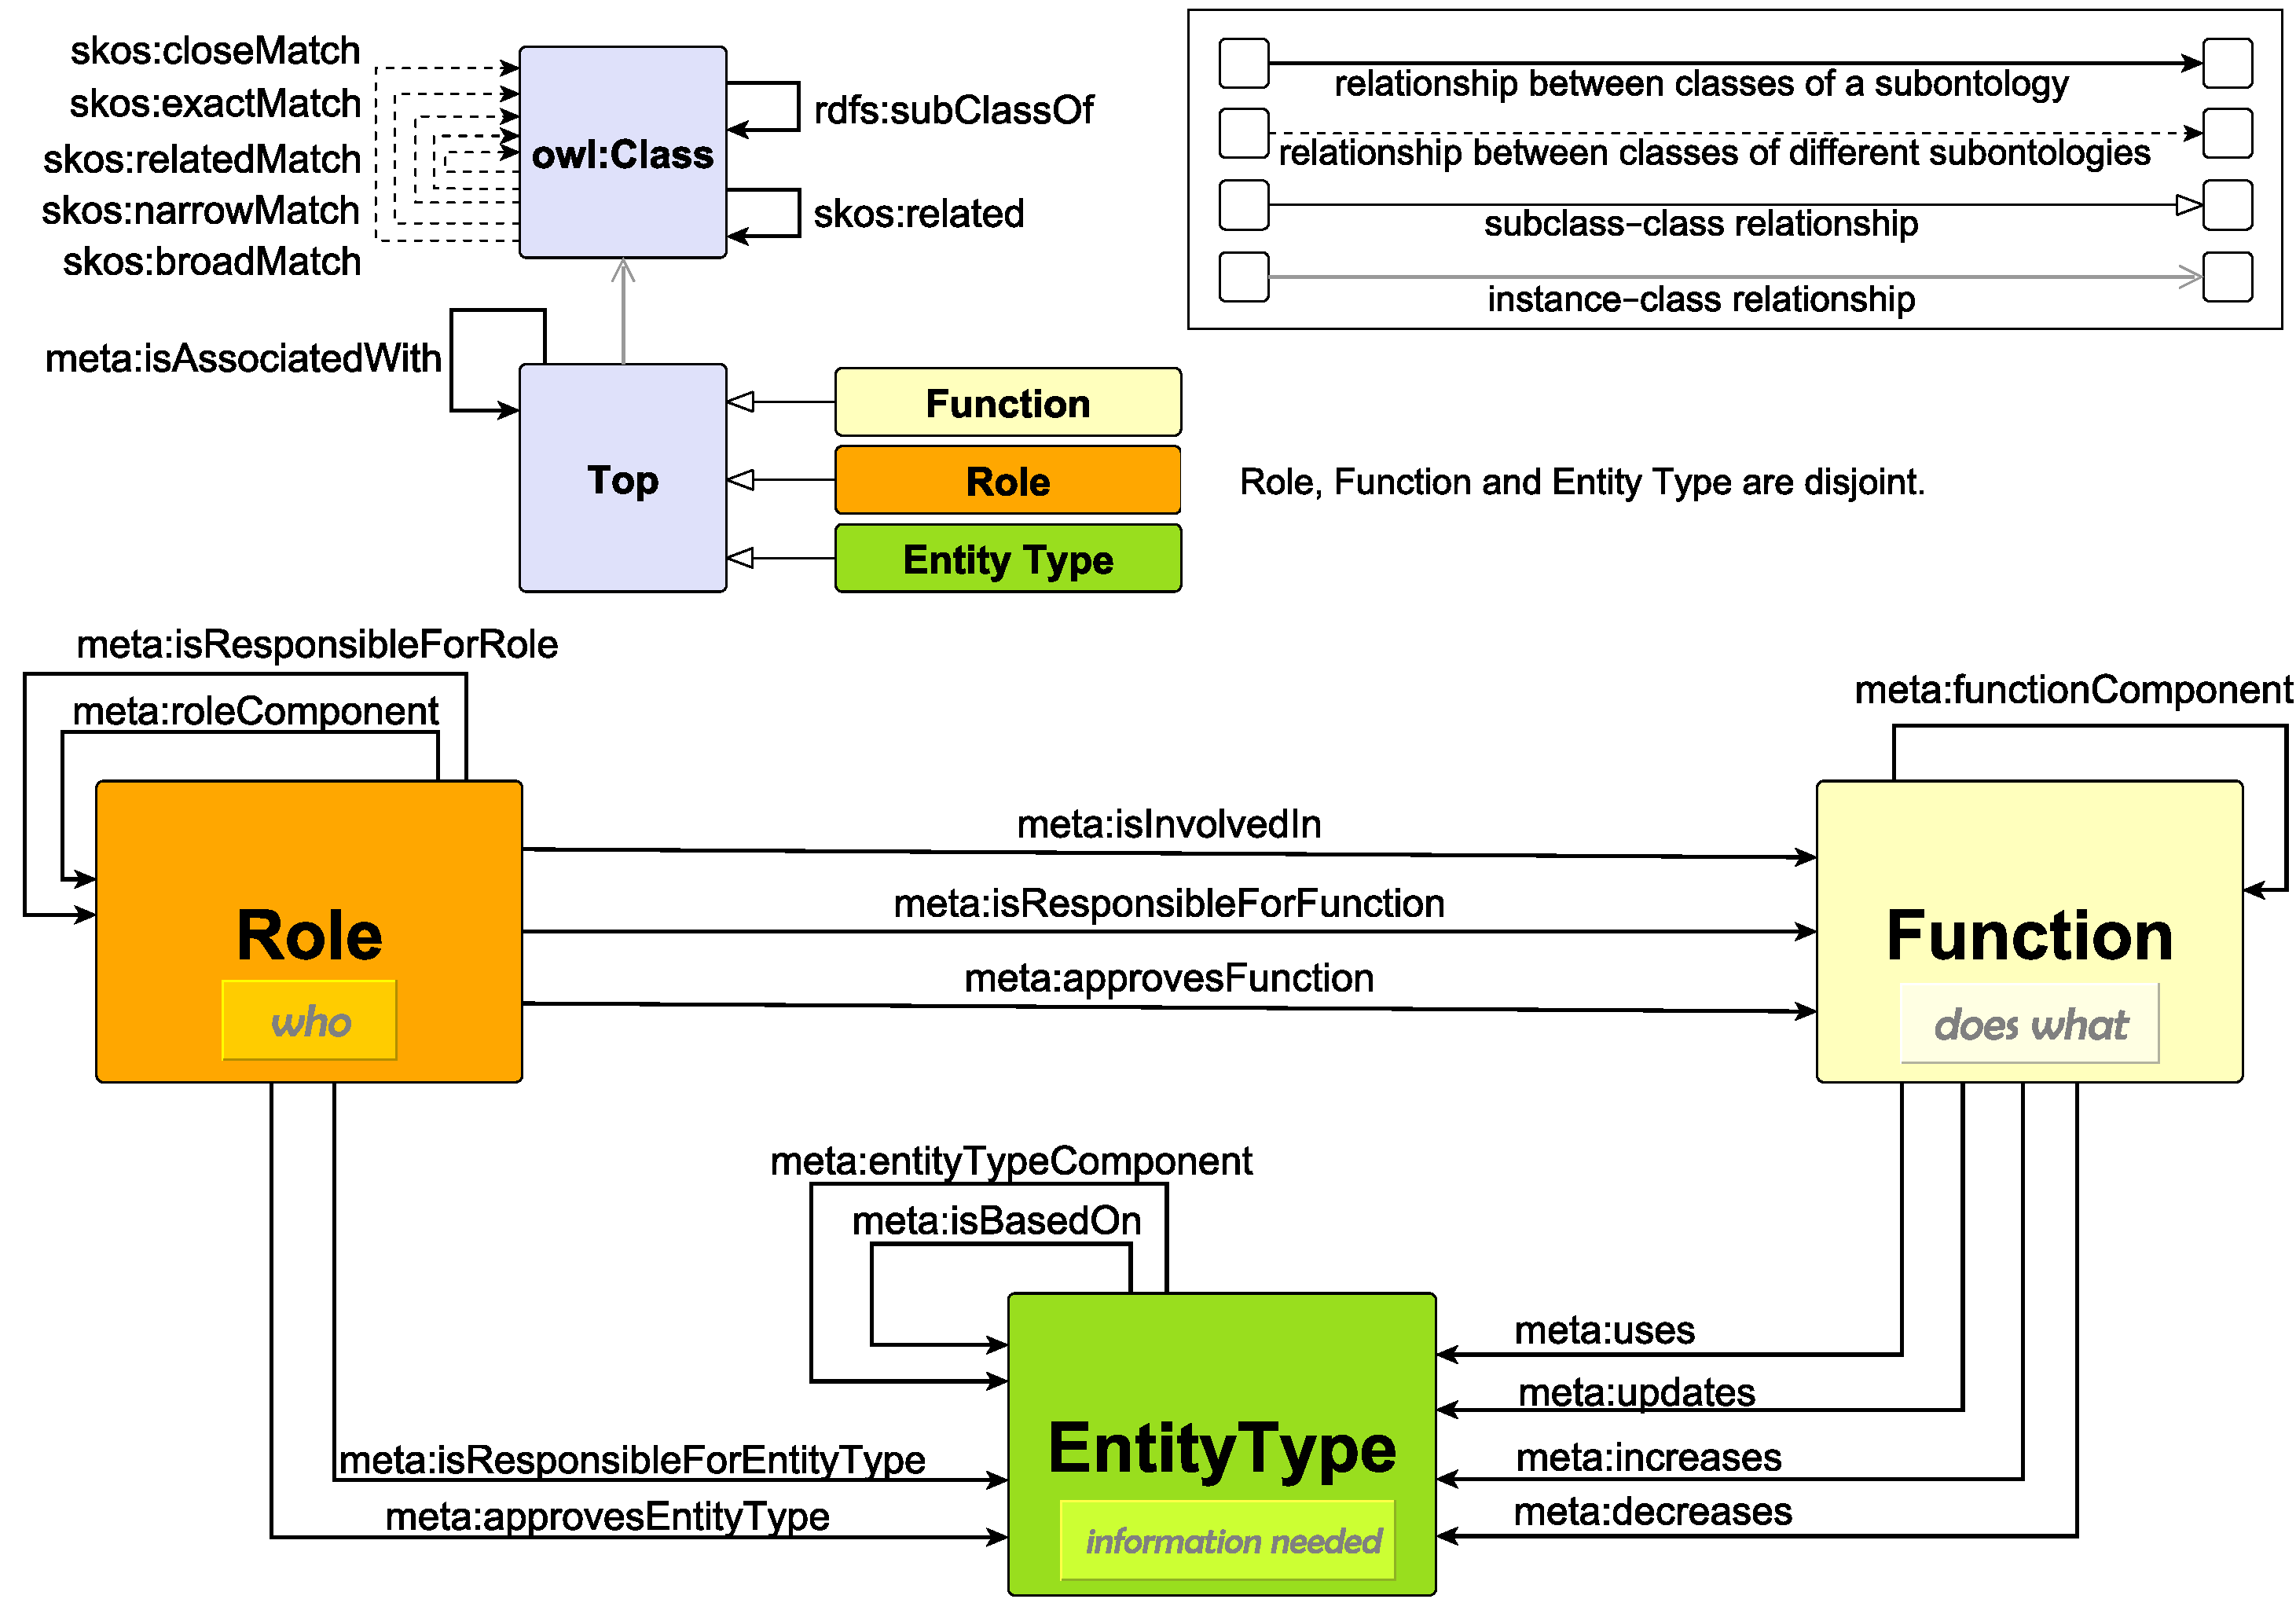
\includegraphics[width=1.01\columnwidth]{img/metamodel9s.pdf}
%\end{minipage}
The Semantic Network of Information Management in Hospitals (SNIK) is an OWL 2 DL ontology with a modular architecture:
The meta model provides a common vocabulary for the domain of hospital information system management.
% and thus defines, which superclasses and relations can be used., see \cref{fig:metamodel}.
It defines three basic disjunctive classes and their relations: Role (who), Function (does what) and Entity Type (and which information is required). %, see \cref{fig:metamodel}.
\vspace{0.3em}
\end{posterbox}
%%%%%%%%%%%%%%%%%%%%%%%%%%%%%%%%%%%%%%%%%%%%%%%%%%%%%%%%%%%%%%%%%%%%%%%%%%%%%%
\begin{posterbox}[name=methods,below=background]{Methods}
Semantic Web technologies and Linked Open Data principles are used to create, store and publish SNIK~\cite{sniktec}.
Subontologies are manually extracted from different sources and build upon the meta model by attaching their subclass hierarchies to the Function, Role and EntityType classes.
{\centering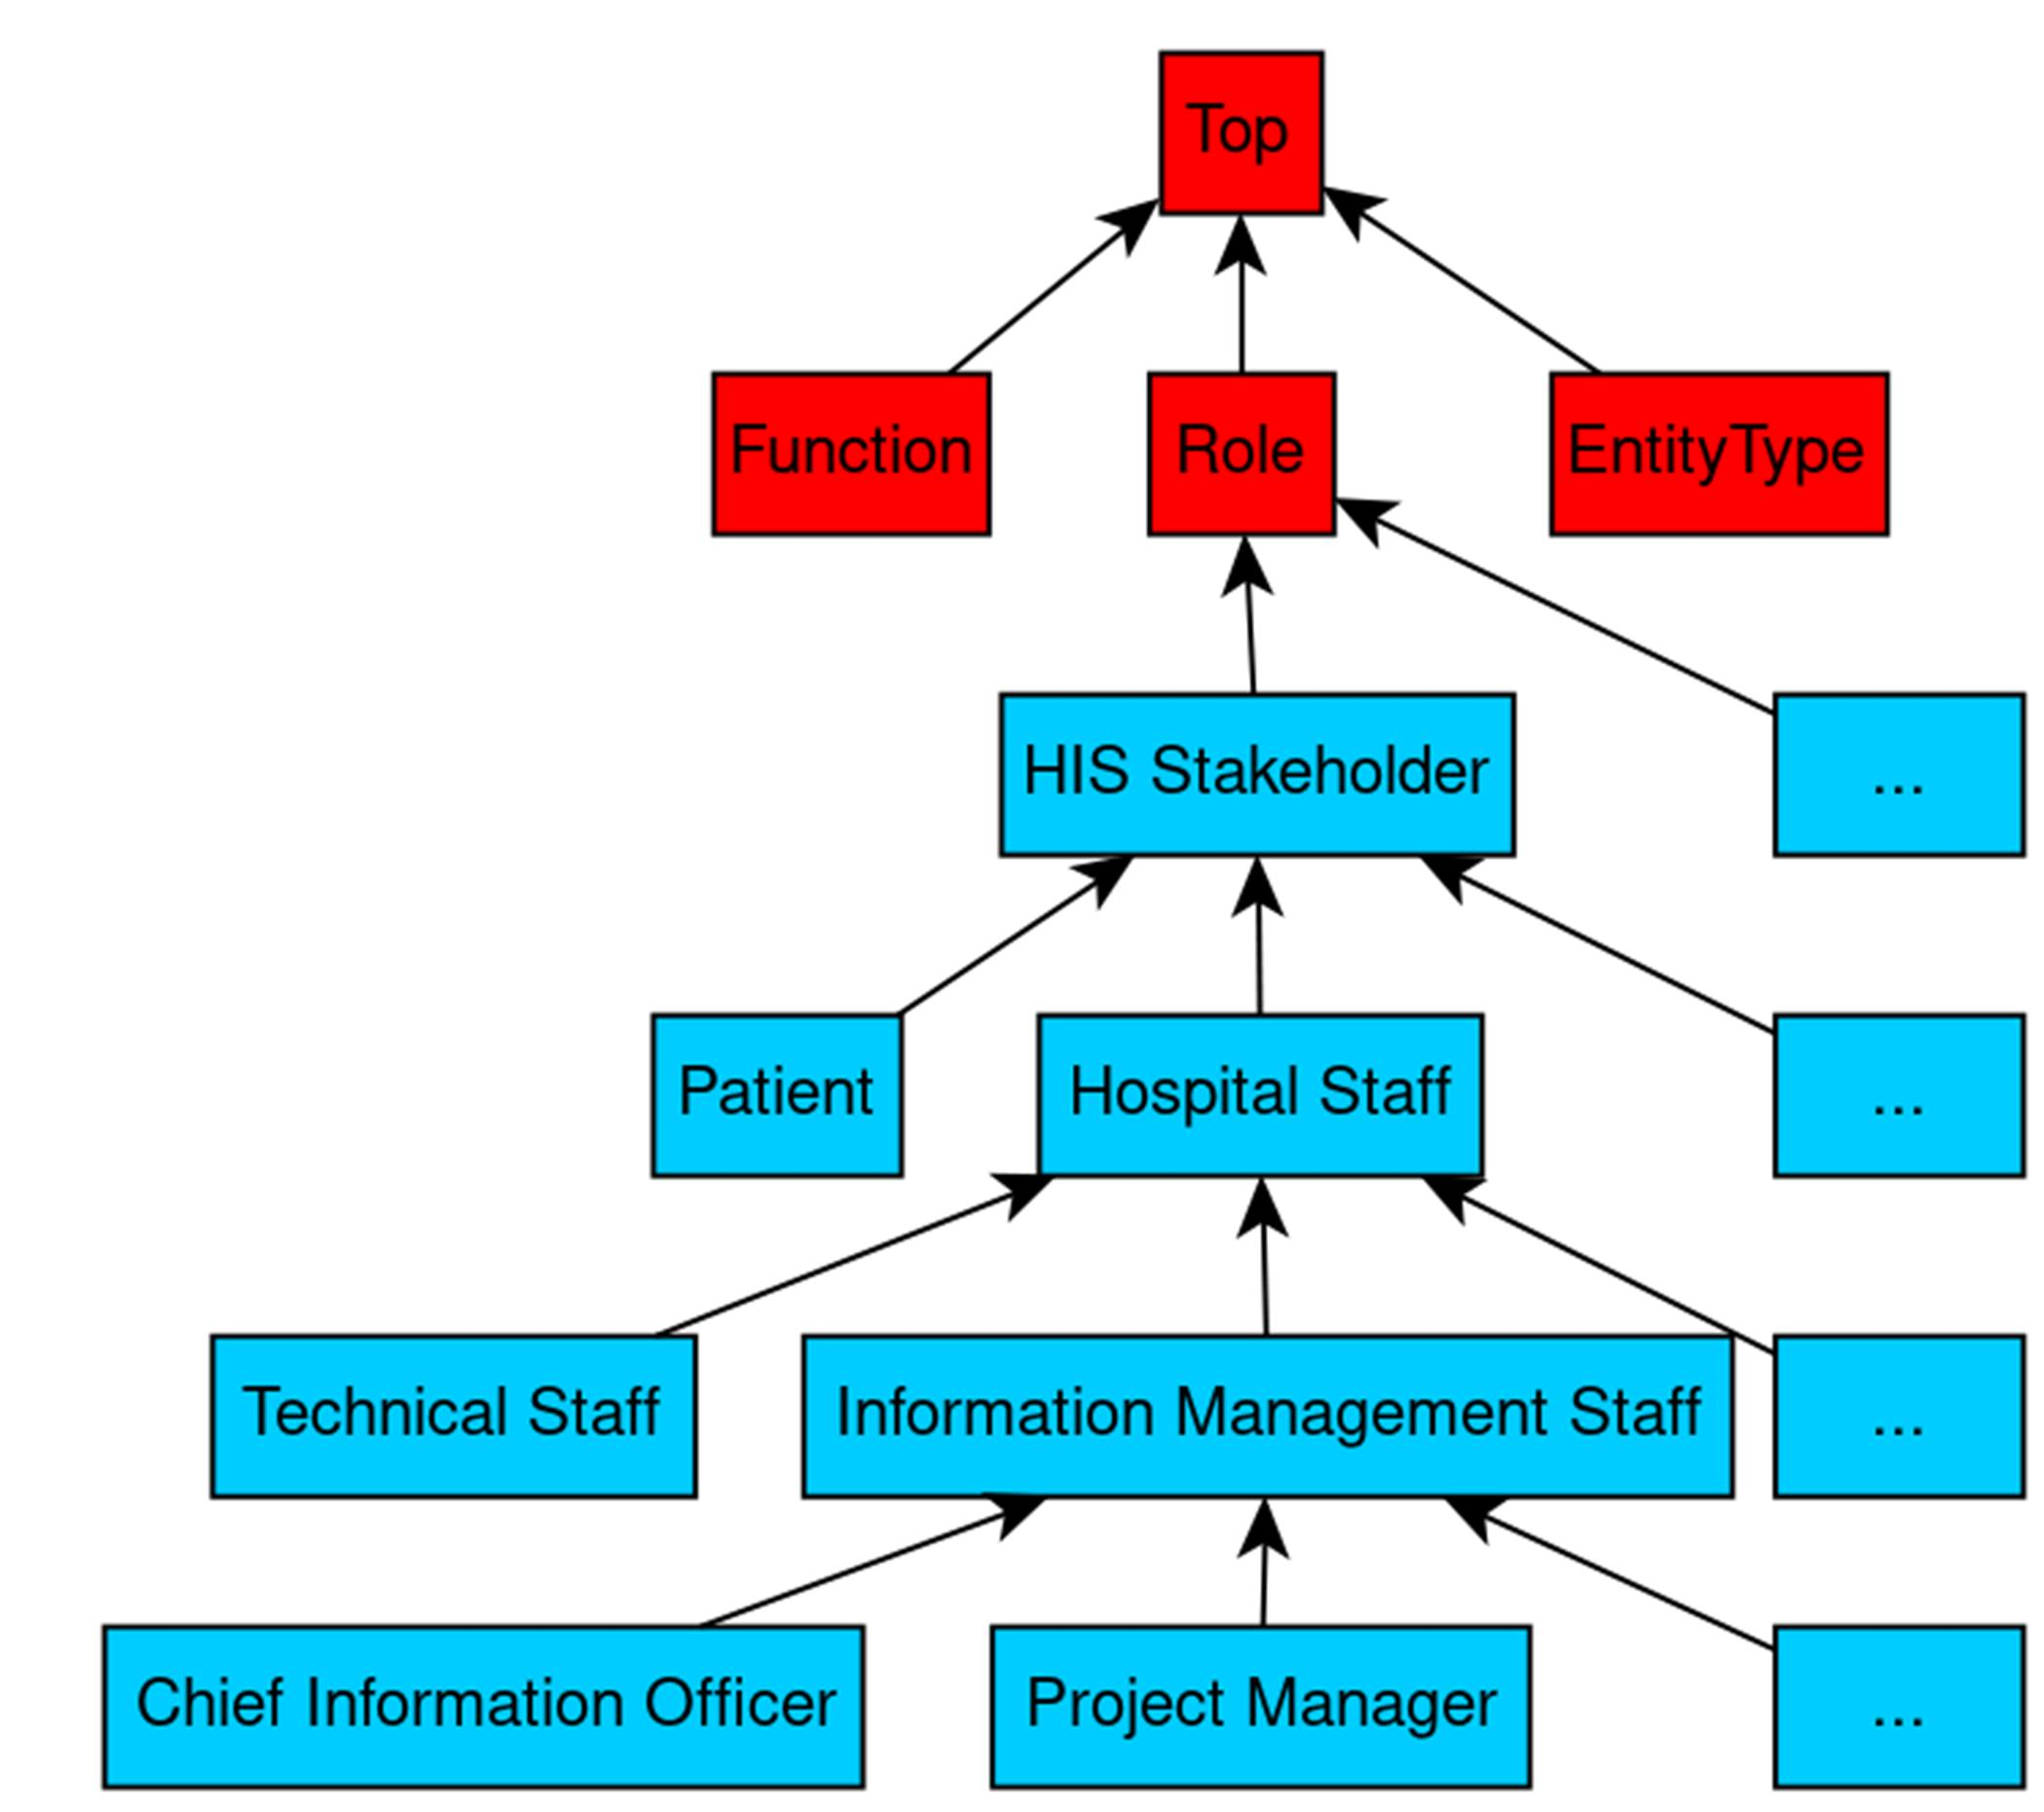
\includegraphics[width=0.8\columnwidth]{img/hierarchy.png}}
\begin{center}
\begin{tabular*}{0.96\columnwidth}{ll}
\toprule
Subontology					&Source\\
\midrule
\url{http://www.snik.eu/ontology/bb}		&Textbook~\cite{bb}\\
\url{http://www.snik.eu/ontology/ob}		&Textbook~\cite{ob}\\
\url{http://www.snik.eu/ontology/he}		&Textbook~\cite{he}\\
\url{http://www.snik.eu/ontology/ciox}		&Hospital CEO Interview\\
\url{http://www.snik.eu/ontology/it4it}		&Standard~\cite{it4it}\\
\bottomrule
\end{tabular*}
\end{center}

%inked Data principles, each class of SNIK has a unique URL.
%We present several interfaces of SNIK that are useful for researchers practitioners and students, depending on their objectives and their semantic web skills.
%resource using the HTTP protocol to receive a description of
%the class, respectively the concept being represented by the
%class, using the standards RDF and SPARQL. Opening a
%We show that those interfaces can benefit teaching, system analysis and integration.
\end{posterbox}
%%%%%%%%%%%%%%%%%%%%%%%%%%%%%%%%%%%%%%%%%%%%%%%%%%%%%%%%%%%%%%%%%%%%%%%%%%%%%%
\begin{posterbox}[name=results,column=1]{Results}
Users can open a SNIK class URL in a web browser to receive a human-readable description using LodLive~\cite{lodlive}:
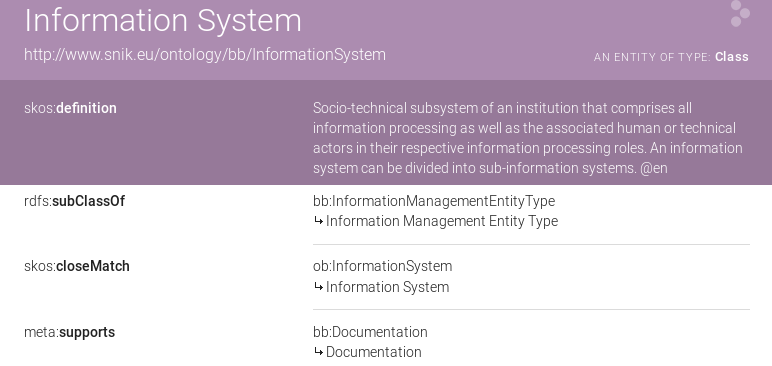
\includegraphics[width=\textwidth]{img/lodlive.png}

\end{posterbox}
%%%%%%%%%%%%%%%%%%%%%%%%%%%%%%%%%%%%%%%%%%%%%%%%%%%%%%%%%%%%%%%%%%%%%%%%%%%%%%
\begin{posterbox}[name=snikgraph,column=1,below=results]{SNIK Graph}
\indent
The most intuitive interface to SNIK is the SNIK Graph visualization, which is based on the Cytoscape.js browser graph library.
SNIK Graph queries the list of classes and their relations from the SPARQL endpoint and transforms them into nodes and edges of the graph.
Exploration options like the “spider worm”, which consists of the shortest path between a start node and an end node together with the end node’s neighbourhood, illustrate the context of a concept.
\vspace{0.3em}
  \end{posterbox}
%%%%%%%%%%%%%%%%%%%%%%%%%%%%%%%%%%%%%%%%%%%%%%%%%%%%%%%%%%%%%%%%%%%%%%%%%%%%%%
\begin{posterbox}[name=sparql,column=1,below=background]{SPARQL}
\noindent
Public access to the meta model and the subontologies via SPARQL queries:

\vspace{1em}
{
\rowcolors{0}{mediblue!20}{white}
\centering
\begin{tabular*}{\columnwidth}{l}
Which components of a healthcare network are not healthcare institutions?\\
\begin{lstlisting}
SELECT ?x {bb:HealthCareNetwork meta:entityTypeComponent ?x.
  MINUS {?x rdfs:subClassOf* bb:HealthCareInstitution.}}
\end{lstlisting}\\
%bb:GovernmentalAuthority\\

How many functions is the CIO responsible for?\\
\begin{lstlisting}
SELECT COUNT(?f) {bb:ChiefInformationOfficer meta:isResponsibleForFunction ?f.}
\end{lstlisting}\\
%15\\

Do transinstitutional health information systems support telemicroscopy?\\
\begin{lstlisting}
ASK {bb:TransinstitutionalHealthInformationSystem meta:supports bb:Telemicroscopy.}
\end{lstlisting}
\end{tabular*}
%True
}
\vspace{0.0em}
\end{posterbox}
%%%%%%%%%%%%%%%%%%%%%%%%%%%%%%%%%%%%%%%%%%%%%%%%%%%%%%%%%%%%%%%%%%%%%%%%%%%%%%
\begin{posterbox}[name=source,column=1,below=snikgraph]{Details}
\begin{tabulary}{\columnwidth}{lL}
\toprule
URL		&\url{http://www.snik.eu/ontology}\\
Version		&2018-10-10, 0.4.1\\
License		&CC BY-NC-SA 4.0\\
SPARQL Endpoint	&\url{http://www.snik.eu/sparql}\\
%Subontologies	&\url{http://www.snik.eu/ontology/bb}\\
%		&\url{http://www.snik.eu/ontology/ciox,}\\
%		&\url{http://www.snik.eu/ontology/ob}\\
%		&\url{http://www.snik.eu/ontology/he}\\
%		&\url{http://www.snik.eu/ontology/it4it}\\
Visualization	&\url{http://www.snik.eu/graph}\\
RDF Browser	&\url{http://www.snik.eu/ontology}\\
Download	&\url{https://github.com/IMISE/snik-ontology/releases/download/0.8.0/snik-0.8.zip}\\
\# Triples	&\num{112747}\\
\# Classes	&\num{4729}\\
\# Properties	&\num{329}\\
\# Interlinks	&\num{713}\\
\bottomrule
\end{tabulary}%The source code for the services is available at \url{https://github.com/imise}
\end{posterbox}
%%%%%%%%%%%%%%%%%%%%%%%%%%%%%%%%%%%%%%%%%%%%%%%%%%%%%%%%%%%%%%%%%%%%%%%%%%%%%%
\begin{posterbox}[name=references,column=1,below=sparql]{References}
    %\smaller
    \bibliographystyle{abbrv}
    \begingroup
    \renewcommand{\section}[2]{}%suppress heading
    \bibliography{poster}
    \endgroup
    \vspace{0.3em}
    %The SNIK project is supported by the DFG (German Research Foundation) under the grant numbers 1605/7-1 and 1387/8-1.
    SNIK is supported under the DFG grant numbers 1605/7-1 and 1387/8-1.
  \end{posterbox}
%%%%%%%%%%%%%%% IMISE Logo
 \node [anchor=south west, inner sep=1pt] at (current page.south west)
 {
\includegraphics[height=0.03\textheight]{img/imise-logo.pdf}
 };
%%%%%%%%%%%%%%% SNIK Logo 
 \node [anchor=south, inner sep=1pt,xshift=-5.5em] at (current page.south) % for unknown reasons the xshift is necessary
 {
\includegraphics[height=0.03\textheight]{img/snik-logo.png}
 };
%%%%%%%%%%%%%%% DFG Logo
 \node [anchor=south east, inner sep=1pt,xshift=-2.5em] at (current page.south east) % for unknown reasons the xshift is necessary
 {
\includegraphics[height=0.03\textheight]{img/dfg-logo.pdf}
 };
%%%%%%%%%%%%%%%%%%%%%%%%%%%%%%%%%%%%%%%%%%%%%%%%%%%%%%%%%%%%%%%%%%%%%%%%%%%%%%
\end{poster}
\end{document}

